\documentclass[a4paper, 12pt]{report}

\usepackage[utf8]{inputenc}
\usepackage{amsfonts, amsmath, amssymb, amsthm}
\usepackage[a4paper, left=4cm, top=3cm, right=3cm, bottom=3cm]{geometry}
\usepackage{graphicx}
\usepackage{tgtermes}
\usepackage[indonesian]{babel}
\usepackage[hidelinks]{hyperref}
\usepackage[notocbib]{apacite}
\usepackage{titlesec}
\usepackage{titling}
\usepackage{titletoc}
\usepackage{setspace}
\usepackage[titles]{tocloft}

\hyphenation{
    di-ma-ti-kan
    di-la-ku-kan
    me-to-de
    meng-gu-na-kan
    ser-ver
    dead-lock
    di-per-lu-kan
    peng-akses-an
    meng-aki-bat-kan
    peng-atur-an
    pem-bangun-an
    di-ha-rap-kan
    meng-gang-gu
    mem-per-ta-han-kan
    bottle-neck
    per-for-mance
    meng-gan-ti-kan
    di-bang-kit-kan
    re-in-force-ment
    su-per-vised
    meng-ha-sil-kan
}

% Document Configuration
\setlength{\footskip}{45pt}

\renewcommand{\thechapter}{\Roman{chapter}}
\addto{\captionsindonesian}{\renewcommand{\chaptername}{\uppercase{BAB}}}
\renewcommand{\baselinestretch}{1.5}
\addto{\captionsindonesian}{\renewcommand{\contentsname}{\uppercase{Daftar Isi}}}
\addto{\captionsindonesian}{\renewcommand{\listfigurename}{\uppercase{Daftar Gambar}}}
\addto{\captionsindonesian}{\renewcommand{\listtablename}{\uppercase{Daftar Tabel}}}
\addto{\captionsindonesian}{\renewcommand{\bibname}{\uppercase{Daftar Pustaka}}}
\addto{\captionsindonesian}{\renewcommand{\appendixname}{Lampiran}}

% \renewcommand{\BBAA}{dan}
\renewcommand{\BBAB}{dan}
\renewcommand{\BOthers}{dkk}

\bibliographystyle{apacite}

\titleformat{\chapter}[display]
{\centering\large\bfseries}
{\uppercase{\chaptertitlename}~\thechapter}
{0pt}
{\uppercase}

\titlespacing*{\chapter}{0pt}{-24pt}{40pt}

\titleformat{\section}[hang]
{\normalsize\bfseries}
{\thesection}
{1em}
{}

\titleformat{\subsection}[hang]
{\normalsize\bfseries}
{\thesubsection}
{1em}
{}

\titlecontents{chapter}[0em]{}{\bfseries\MakeUppercase\chaptertitlename~\thecontentslabel\ \MakeUppercase}{\bfseries}{\bfseries\titlerule*[0.8pc]{.}\contentspage}

\titlecontents{figure}[0em]{}{\figurename~\thecontentslabel\quad}{\bfseries}{\titlerule*[0.8pc]{.}\contentspage}

\titlecontents{table}[0em]{}{\tablename~\thecontentslabel\quad}{\bfseries}{\titlerule*[0.8pc]{.}\contentspage}

% Daftar Lampiran
\newcommand{\listappendixname}{\MakeUppercase{Daftar Lampiran}}
\newlistof{appendix}{app}{\listappendixname}

\newcommand{\appendixchapter}[1]{
    \chapter{#1}
    \addcontentsline{app}{appendix}{\protect\bfseries\MakeUppercase{Lampiran~\numberline{\thechapter.}#1}}\par
}
\newcommand{\appendixsection}[1]{
    \section{#1}
    \addcontentsline{app}{appendix}{\protect\hspace{1.5em}\thesection\quad#1}\par
}

% CONTENT 
\title{$<$CONTOH JUDUL: PERANCANGAN ANTARMUKA SISTEM INFORMASI DI PUSKESMAS DAERAH PEDESAAN MENGGUNAKAN USER CENTERED DESIGN$>$}
\author{$<$NAMA MAHASISWA$>$ \\ NIM: $<$NIM MAHASISWA$>$}
\date{}

\begin{document}

\pagestyle{empty}
\begin{center}
    \bfseries\large\MakeUppercase{\thetitle}

    \vspace{5em}

    \bfseries\normalsize{Disusun sebagai syarat kelulusan mata kuliah\\ 
    IF4091/Penyusunan Proposal}

    \vspace{5em}
    
    \bfseries{\normalsize{Oleh}\\ \large{\theauthor}}

    \vspace{4.5em}

    
\includegraphics[scale=0.1]{images/gajah_itb_transparan_syeilendra.png}

    \vspace{3em}
    \large{\bfseries{\MakeUppercase{Program Studi Teknik Informatika\\
        Sekolah Teknik Elektro \& Informatika\\
        Institut Teknologi Bandung}\\$<$Bulan$>$ $<$Tahun$>$}}
    
\end{center}
\clearpage

\pagestyle{plain}
\pagenumbering{gobble}
\begin{center}
    \large{\MakeUppercase{\bfseries\thetitle}}

    \vspace{5em}

    \large{\bfseries Laporan Proposal Tugas Akhir}

    \vspace{3em}
    
    \normalsize{\textbf{Oleh}}\\ 
    \large{\bfseries \theauthor \\ Program Studi Teknik Informatika}\\
    
    \normalsize{Sekolah Teknik Elektro dan Informatika \\ Institut Teknologi Bandung}

    \vspace{5em}

    Bandung, $<$tanggal$>$\\

    Mengetahui,\\

    \vspace{2em}
    
    Pembimbing,\\

    \vspace{6em}

    \underline{$<$Nama Pembimbing$>$}\\
    NIP. $<$NIP Pembimbing$>$
    
\end{center}

\pagenumbering{arabic}
\setcounter{page}{1}
\tableofcontents

\listofappendix

\listoffigures

\listoftables
\newpage

\chapter{Pendahuluan}
Bab Pendahuluan secara umum yang dijadikan landasan kerja dan arah kerja penulis tugas akhir, berfungsi mengantar pembaca untuk membaca laporan tugas akhir secara keseluruhan.

\section{Latar Belakang}
Latar Belakang berisi dasar pemikiran, kebutuhan atau alasan yang menjadi ide dari topik tugas akhir. Tujuan utamanya adalah untuk memberikan informasi secukupnya kepada pembaca agar memahami topik yang akan dibahas. Saat menuliskan bagian ini, posisikan anda sebagai pembaca – apakah anda tertarik untuk terus membaca?

\section{Rumusan Masalah}
Rumusan masalah yang baik memiliki struktur sebagai berikut:
\begin{enumerate}
    \item Penjelasan ringkas tentang kondisi/situasi yang ada sekarang terkait dengan topik utama yang dibahas Tugas Akhir.
    \item Pokok persoalan dari kondisi/situasi yang ada, dapat dilihat dari kelemahan atau kekurangannya. Bagian ini merupakan inti dari rumusan masalah.
    \item Elaborasi lebih lanjut yang menekankan pentingnya untuk menyelesaikan pokok persoalan tersebut.
    \item Usulan singkat terkait dengan solusi yang ditawarkan untuk menyelesaikan persoalan.
\end{enumerate}

Penting untuk diperhatikan bahwa persoalan yang dideskripsikan pada subbab ini akan dipertanggungjawabkan di akhir pelaksanaan tugas akhir apakah terselesaikan atau tidak.

\section{Tujuan dan Ukuran Keberhasilan Pencapaian}
Tuliskan tujuan utama dan/atau tujuan detil yang akan dicapai dalam pelaksanaan tugas akhir. Fokuskan pada hasil akhir yang ingin diperoleh setelah tugas akhir diselesaikan, terkait dengan penyelesaian persoalan pada rumusan masalah. Penting untuk diperhatikan bahwa tujuan yang dideskripsikan pada subbab ini akan dipertanggungjawabkan di akhir pelaksanaan tugas akhir apakah tercapai atau tidak. Tuliskan juga ukuran keberhasilan pencapaiannya.

\section{Batasan Masalah}
Tuliskan batasan-batasan yang diambil dalam pelaksanaan tugas akhir. Batasan ini dapat dihindari (tidak perlu ada) jika topik/judul tugas akhir dibuat cukup spesifik.

\section{Metodologi}
Tuliskan semua tahapan yang akan dilalui selama pelaksanaan tugas akhir. Tahapan ini spesifik untuk menyelesaikan persoalan tugas akhir. Tahapan studi literatur tidak perlu dituliskan karena ini adalah pekerjaan yang harus Anda lakukan selama proses pelaksanaan tugas akhir.
\chapter{Kajian Pustaka}

Bab Kajian Pustaka digunakan untuk mendeskripsikan kajian literatur yang terkait dengan persoalan tugas akhir. Tujuan kajian pustaka adalah:
\begin{enumerate}
\item memberikan pemahaman yang cukup kepada pembaca tentang teori atau pekerjaan yang terkait langsung dengan penyelesaian persoalan

\item menyampaikan informasi apa saja yang sudah ditulis/dilaporkan oleh pihak lain (peneliti/Tugas Akhir/Tesis) tentang hasil penelitian/pekerjaan mereka yang sama/mirip/erat kaitannya dengan persoalan tugas akhir

\item menunjukkan kepada pembaca adanya gap seperti pada rumusan masalah yang memang belum terselesaikan
\end{enumerate}

\section{Contoh Subbab}
Contoh subbab

\subsection{Contoh Subbab}
Contoh subbab.

\subsubsection{Contoh Gambar dan Tabel}
Contoh gambar adalah sebagaimana terlihat pada Gambar \ref{fig:eg}.
\begin{figure}
    \centering
    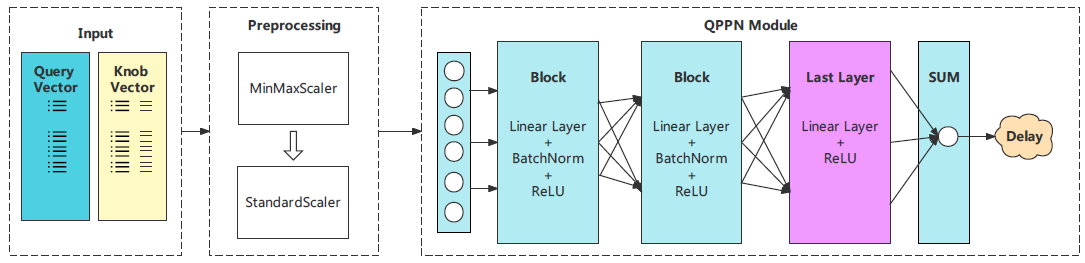
\includegraphics[width=0.8\linewidth]{images/QPPN.png}
    \caption{Tahapan konstruksi koleksi retorik kalimat}
    \label{fig:eg}
\end{figure}

Contoh tabel adalah sesuai yang terlihat pada Tabel \ref{tab:my_label}.
\begin{table}[]
    \centering
    \begin{tabular}{|l|l|}
    \hline
    Nomor \textit{Tag}  & Keterangan \\
    \hline
        0xx  & Kendali informasi, nomor dan kode\\
        \hline
        1xx & Main entry\\
    \hline
    \end{tabular}
    \caption{Pengelompokan \textit{Tag} MARC-21}
    \label{tab:my_label}
\end{table}
\chapter{ANALISIS MASALAH DAN RANCANGAN SOLUSI}

Tujuan utama penulisan bab ini adalah untuk menguraikan rencana penyelesaian masalah tugas akhir I.. Bab ini mencakup antara lain:

\begin{enumerate}

    \item Deskripsi dan analisis persoalan yang terkait dengan Rumusan Masalah, misalnya menjelaskan secara detail latar belakang dan masalah yang menjadi dasar munculnya topik, menunjukkan gap/celah antara kondisi saat ini dengan kondisi yang diharapkan, dan kaitan antara sistem/aplikasi yang dikembangkan dengan sistem/aplikasi lain yang terkait.

    \item Analisis solusi yang terdiri dari pilihan alternatif solusi yang dapat digunakan untuk setiap permasalahan berdasarkan hasil studi literatur atau survei, pemilihan solusi beserta justifikasinya.

    \item Deskripsi umum solusi yang dipilih, mencakup:
    \begin{enumerate}
        \item Modul/subsistem/komponen yang akan dikembangkan untuk menyelesaikan masalah, berikut penjelasannya.
        \item Alur umum algoritma atau langkah-langkah pengembangan sistem dan penjelasannya.
        \item Penggunaan kakas yang diperlukan
    \end{enumerate}
\end{enumerate}

Dianjurkan untuk menggunakan diagram sebagai pendukung penjelasan bagian ini.
\chapter{Rencana Pelaksanaan}
Bab Rencana Pelaksanaan digunakan untuk mendeskripsikan rencana pelaksanaan berupa jadwal dan risiko-risiko yang mungkin dihadapi dan rencana mitigasinya. Tujuan bab ini adalah:
\begin{enumerate}
\item Mahasiswa memiliki rencana yang jelas mengenai pelaksanaan TA

\item Mahasiswa mengenali risiko-risiko yang mungkin dihadapi dan sudah menyiapkan diri untuk mengantisipasi risiko tersebut.
\end{enumerate}

\section{Jadwal}
Cantumkan jadwal pengerjaan tugas akhir lengkap dengan uraiannya.

\section{Risiko}
Cantumkan 5 risiko tertinggi yang mungkin dihadapi dalam pengerjaan tugas akhir. Risiko yang dicantumkan dapat merupakan risiko dari sisi teknis, risiko dari sisi operasional, risiko dari metode yang dipilih, dan sebagainya. Cantumkan pula rencana mitigasi dari risiko-risiko tersebut.

\begingroup
\setstretch{1.0}
\bibliography{references/references}
\endgroup

\appendix

\addtocontents{toc}{\protect\setcounter{tocdepth}{-1}}
\titleformat{\chapter}[block]
{\large\bfseries}
{\chaptertitlename~\thechapter.~}
{0pt}
{}

\appendixchapter{Contoh Judul Lampiran}

\appendixsection{Contoh Judul Anak Lampiran}
Contoh anak lampiran
\end{document}